\documentclass[12pt, varwidth, border=5mm]{standalone}
\usepackage{tikz}
\usepackage{amsmath}
% Underlining package
\usepackage{ulem}
\usetikzlibrary{angles,quotes}
\usetikzlibrary{intersections}
\usetikzlibrary{arrows.meta}
\usetikzlibrary{calc}
% \usepackage[a4paper, portrait, margin=1cm]{geometry}


\begin{document}
\section*{ }
    
$\text{e} = \text{\dotuline{~~~~~~~}}^\circ$
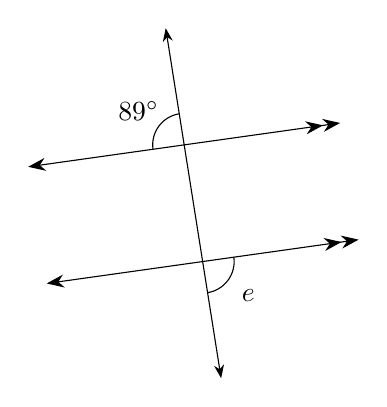
\begin{tikzpicture}[scale=1.0, baseline=(current bounding box.north)]
  \begin{scope}[rotate=279]
    % Draw the first line
    \draw[<->>, >={Stealth[scale=1.3]}, name path=P1] (0, 0) -- (0.0698096257491344, 3.999390780625565);
    % Draw the second line with the calculated offsets
    \draw[<->>, >={Stealth[scale=1.3]}, name path=P2] (1.5002284920658615, 0) -- (1.5700381178149958, 3.999390780625565);
    % Draw the transversal through the middle of the parallel lines
    \draw[<->, >=Stealth, name path=P3] (-1.465095187125433, 1.9996953903127825) -- (3.0351333049404285, 1.9996953903127825);
    \path [name intersections={of=P1 and P3,by=A}];
    \path [name intersections={of=P2 and P3,by=B}];
    % Draw the angle
    \coordinate (p1s) at (0, 0);
    \coordinate (p1e) at (0.0698096257491344, 3.999390780625565);
    \coordinate (p2s) at (1.5002284920658615, 0);
    \coordinate (p2e) at (1.5700381178149958, 3.999390780625565);
    \coordinate (ts) at (-1.465095187125433, 1.9996953903127825);
    \coordinate (te) at (3.0351333049404285, 1.9996953903127825);
    \draw pic["$e$", draw=black, -, angle eccentricity=1.8, angle radius=0.4cm] {angle=te--B--p2e};
\draw pic["$89^\circ$", draw=black, -, angle eccentricity=1.8, angle radius=0.4cm] {angle=ts--A--p1s};

  \end{scope}
\end{tikzpicture}

\end{document}
